\documentclass[a4paper,french]{paper}
\usepackage{../../_latex_assets/villemejane_iogs_ceti}

%Informations about this document 
%------------------------------------------
\def\module{Conception Electronique pour le Traitement de l'Information}
\def\moduleAbrege{5N-027-SCI / CéTI}
\def\annee{}

\def\titre{Bloc 2 / Filtrage actif}
\author{Julien VILLEMEJANE}

\subtitle{Bloc 2}
\institution{LEnsE / Institut d'Optique Graduate School}

\title{\titre}
\begin{document} 
%Beginning First Page. 
%------------------------------------------
\enteteThematiqueObligatoire{}

%Beginning Content. 
%------------------------------------------

\vspace{-1cm}
%%%%%%%%%%%%%%%%%%%
%%%%%%%%%%%%%%%%%%%
%%%%%%%%%%%%%%%%%%%
%%%%%%%%%%%%%%%%%%%
\encadreTDExo{2.1 - Filtrer des composantes fréquentielles - Ordre 1 Passif}{
Proposer une structure de filtre du premier ordre qui laisse passer des signaux au dessus d'une fréquence $f_c$. Donner les principales caractéristiques et limitations d'un tel filtre.
}

Pour réaliser un tel système, on va se baser sur un circuit incluant une résistance et une capacité en série.

\begin{center}
\begin{circuitikz}
	\draw (0,0) to [C=$C$, o-*] (3,0)
		to[R=$R$, -*, i=$I$] (3,-3)
		to[short, -*](1,-3)
		node[ground](GND){}
		to[short, -o](0,-3);
	\draw (3,0) to[short, -o, i=$I_S$](4,0);
	\draw (3,-3) to[short, -o](4,-3);
	% fleche
	\draw (0,-2.7) edge[->] (0,-0.3);
	\node (Ein) at (-0.5,-1.5){$V_E$};
	% fleche
	\draw (4,-0.3) edge[<-, green!40!black] (4,-2.7); 
	\node[text=green!40!black] (US) at (4.5,-1.5){$V_S$};
\end{circuitikz}
\end{center}

On supposera que $I_S = 0$ pour le reste de l'étude (sinon, voir Mission 1.1).

On se placera également en \textbf{régime harmonique} (réponse en fréquence) dans cette étude. Il est en effet possible de traiter ce problème en \textit{régime transitoire}, basé sur l'étude temporelle.

\medskip

Loi des mailles du circuit :

\begin{enumerate}
	\item $V_S - R \cdot I = 0$
	\item $V_E - \frac{I}{j \cdot C \cdot \omega} - V_S$  (où $j^2 = -1$ et $\omega$ est la pulsation des signaux électriques
\end{enumerate}

D'après (1), on obtient $I = \frac{V_S}{R}$.

En remplaçant $I$ dans (2), on obtient : $V_E = V_S \cdot (1 + \frac{1}{j \cdot R \cdot C \cdot \omega}$

Ainsi, on obtient la fonction de transfert suivante : 
$$\boxed{ H(j \cdot \omega) = \frac{V_S}{V_E} = \frac{j \cdot R \cdot C \cdot \omega}{1 + j \cdot R \cdot C \cdot \omega} }$$

On posera $\omega_0 = \frac{1}{R \cdot C}$, appelée aussi \textbf{pulsation caractéristique} de ce système. 

Dans le cas d'un circuit du premier ordre, il s'agit également de la limite de la bande-passante à $-3\operatorname{dB}$.

\noindent\hrulefill

\textbf{Etude en fréquence}

Il est alors possible d'étudier la réponse de ce montage en fonction de la fréquence $f$ du signal d'entrée (ou de sa pulsation $w = 2 \cdot \pi \cdot f$).

Afin de simplifier l'étude de la mise en cascade de filtres, il est courant de passer dans une échelle logarithmique.

Lors de la mise en série de systèmes de ce type, les fonctions de transfert se multiplient. Le passage en logarithme permet alors d'additionner l'ensemble des fonctions de transfert... ($\log{H_1 \cdot H_2} = \log{H_1} + \log{H_2}$).

On calcule alors le gain en décibels du système par la relation : $$\boxed{G_{dB} = 20 \cdot \log{ \mid H \mid }}$$.

\medskip

Il est possible à ce stade d'utiliser des outils numériques (voir ONIP-1 - Bloc 1) pour automatiser l'étude de systèmes de ce type et générer les graphiques.

En Python, par exemple, il est possible d'utiliser le module \textit{control} qui permet de traiter des systèmes.

Le code suivant permet de définir un système du premier ordre de type passe-haut et d'afficher la réponse en fréquence (diagramme de Bode - gain et phase).

\begin{lstlisting}
import control
import numpy as np

#%% System definition - high-pass first order
w0 = 1e3
num = np.array([1/w0, 0])
den = np.array([1/w0, 1])

system = control.tf(num, den)
display(system)

#%% Diagramme de Bode
omega = np.logspace(1, 5, 101)
control.bode_plot(system, omega=omega, Hz=True, dB=True)
\end{lstlisting}

On obtient alors le graphique suivant :

\begin{center}
	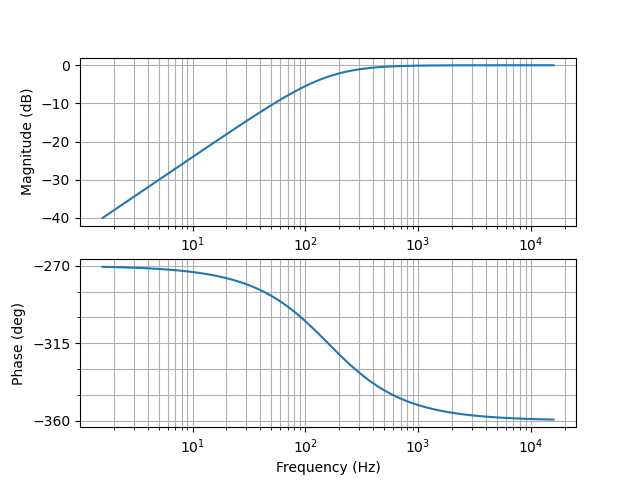
\includegraphics[width=12cm]{images/rc_filter_bode.png}
\end{center}

On peut noter que les hautes fréquences (à droite du graphique) sont bien conservées (gain de $0\operatorname{dB}$) alors que les basses fréquences (à gauche) sont très fortement atténuées.

\newpage
\textbf{Etude en régime transitoire / temporel}

Il est également possible d'étudier la réponse de ce filtre en temporel.

\begin{center}
\begin{circuitikz}
	\draw (0,0) to [C=$C$, o-*] (3,0)
		to[R=$R$, -*, i=$i(t)$] (3,-3)
		to[short, -*](1,-3)
		node[ground](GND){}
		to[short, -o](0,-3);
	\draw (3,0) to[short, -o, i=$i_S$](4,0);
	\draw (3,-3) to[short, -o](4,-3);
	% fleche
	\draw (0,-2.7) edge[->] (0,-0.3);
	\node (Ein) at (-0.5,-1.5){$v_E(t)$};
	% fleche
	\draw (4,-0.3) edge[<-, green!40!black] (4,-2.7); 
	\node[text=green!40!black] (US) at (4.5,-1.5){$v_S(t)$};
\end{circuitikz}
\end{center}

On peut écrire les lois suivantes :

\begin{enumerate}
	\item $v_S(t) = R \cdot i(t)$
	\item $i = C \cdot \frac{d (v_S - v_E) }{dt}$
\end{enumerate}

On obtient alors l'équation suivante : $$\boxed{v_S - R \cdot C \cdot \frac{dv_S}{dt} + R \cdot C \cdot \frac{dv_E}{dt} = 0}$$

Equation différentielle du premier ordre à résoudre.

\newpage
%%%%%%%%%%%%%%%%%%%
%%%%%%%%%%%%%%%%%%%
%%%%%%%%%%%%%%%%%%%
%%%%%%%%%%%%%%%%%%%
\encadreTDExo{2.2 - Filtrer des composantes fréquentielles - Ordre 2}{
On se propose d'étudier la structure suivante :

\begin{center}
	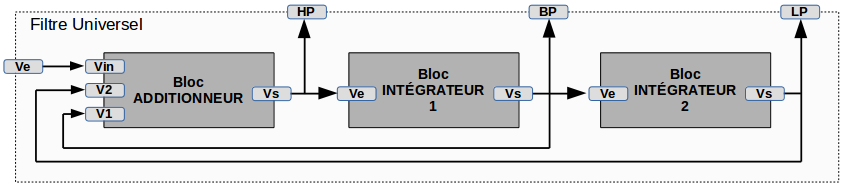
\includegraphics[width=14cm]{images/universel_structure.png}
\end{center}

Pour cela, on se propose d'étudier les deux circuits suivants :

\begin{center}
	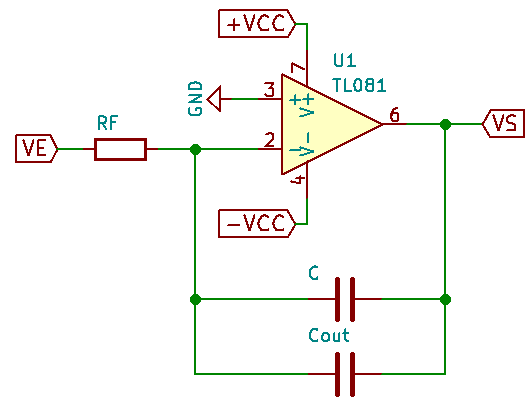
\includegraphics[width=7cm]{images/universel_integrateur.png}
	\quad
	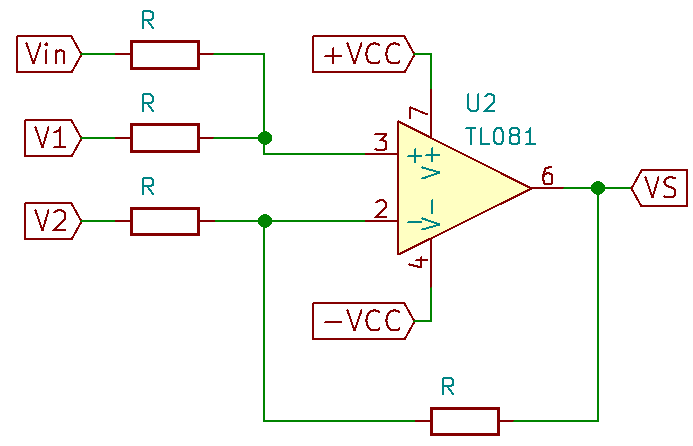
\includegraphics[width=7cm]{images/universel_sommateur.png}
\end{center}
}

Dans la suite de l'étude, on fera l'hypothèse d'ALI parfaits où $i^+ = i^- = 0$.

On prendra également comme convention pour les courants positifs ceux allant de l'extérieur du circuit vers l'entrée de l'ALI.

\textbf{Etude de l'additionneur}

On remarque une contre-réaction entre la sortie ($V_S$) et l'entrée inverseuse ($V^-$) par l'intermédiaire de la résistance $R$. On peut alors faire l'hypothèse d'un régime linéaire de fonctionnement et ainsi $V^+ = V^-$.

\medskip

\textbf{\textit{Calcul de $V^+$}}

Lois appliquées autour de $V^+$ :
\begin{enumerate}
	\item $I_{In} + I_1 = 0$ (loi des noeuds)
	\item $I_{In} = \frac{(V_{In} - V^+)}{R}$ (loi d'Ohm)
	\item $I_{1} = \frac{(V_{1} - V^+)}{R}$ (loi d'Ohm)
\end{enumerate}

A partir de l'équation (1), on obtient : $I_{In} = - I_1$

Et ainsi :
$$\frac{(V_{In} - V^+)}{R} = - \frac{(V_{1} - V^+)}{R}$$

On obtient alors : $$\boxed{V^+ = \frac{V_{In} + V_1}{2}}$$

\textbf{\textit{Calcul de $V^-$}}

Lois appliquées autour de $V^-$ :
\begin{enumerate}
	\item $I_{S} + I_2 = 0$ (loi des noeuds)
	\item $I_{2} = \frac{(V_{2} - V^-)}{R}$ (loi d'Ohm)
	\item $I_{S} = \frac{(V_{S} - V^-)}{R}$ (loi d'Ohm)
\end{enumerate}

A partir de l'équation (1), on obtient : $I_{S} = - I_2$

Et ainsi :
$$\frac{(V_{2} - V^-)}{R} = - \frac{(V_{S} - V^-)}{R}$$

On obtient alors : $$\boxed{V^- = \frac{V_{S} + V_2}{2}}$$

\textbf{\textit{Montage complet}}

En appliquant l'hypothèse $V^+ = V^-$, on obtient alors : $$\boxed{V_S = V_{In} + V_1 - V_2}$$

\newpage

\textbf{Etude de l'intégrateur}

On remarque là encore une contre-réaction entre la sortie ($V_S$) et l'entrée inverseuse ($V^-$) par l'intermédiaire des capacités $C$ et $C_{out}$, qui sont des éléments linéaires. On peut alors faire l'hypothèse d'un régime linéaire de fonctionnement et ainsi $V^+ = V^-$.

\textbf{\textit{Calcul de $V^-$}}

Lois appliquées autour de $V^-$ :
\begin{enumerate}
	\item $I_{E} + I_{S} = 0$ (loi des noeuds)
	\item $I_{E} = \frac{(V_{E} - V^-)}{R_F}$ (loi d'Ohm)
	\item $I_{S} = \frac{(V_{S} - V^-)}{Z_{eq}}$ (loi d'Ohm)
\end{enumerate}

$Z_{eq}$ est l'impédance équivalente de la mise en parallèle des deux capacités $C$ et $C_{out}$.

On peut alors écrire : $\frac{1}{Z_{eq}} = \frac{1}{Z_C} + \frac{1}{Z_{Cout}}$

On obtient alors : $Z_{eq} = j \cdot (C + C_{out}) \cdot \omega$

\medskip

A partir de l'équation (1), on obtient : $I_{S} = - I_{E}$

Et ainsi :
$$\frac{(V_{E} - V^-)}{R_F} = - \frac{(V_{S} - V^-)}{Z_{eq}}$$

\medskip

On obtient alors au final la fonction de transfert suivante : 
$$\boxed{H = \frac{V_S}{V_E} = \frac{1}{j \cdot R_F \cdot (C + C_{out}) \cdot \omega}}$$

\newpage

\textbf{Etude du filtre universel}

Si on s'intéresse à présent à la structure complète, on voit que :
\begin{enumerate}
	\item $V_1 = V_{BP} = V_{HP} / (j \cdot R_F \cdot (C + C_{out}) \cdot \omega)$ (intégrateur)
	\item $V_2 = V_{LP} = V_{BP} / (j \cdot R_F \cdot (C + C_{out}) \cdot \omega)$ (intégrateur)
	\item $V_{Sadd} = V_{HP} = V_E + V_1 - V_2 = V_E + V_{BP} - V_{LP}$
\end{enumerate}

Des deux premières équations, on peut en découler que $V_{LP} = V_{HP} / (j \cdot R_F \cdot (C + C_{out}) \cdot \omega)^2$ (double intégration)

\medskip

Pour la suite, on posera $\omega_c = \frac{1}{R_F \cdot (C + C_{out})}$.

Ainsi, on obtient la relation suivante entre $V_E$ et $V_{HP}$ :
$$ V_{HP} = V_E + \frac{V_{HP}}{j \cdot \omega / \omega_c} - \frac{V_{HP}}{(j \cdot \omega / \omega_c)^2}$$

\medskip

Après remise en forme de cette expression, on trouve alors :
$$\boxed{ H_{HP} = \frac{V_{HP}}{V_E} = \frac{(j \cdot \omega / \omega_c)^2}{1 - (j \cdot \omega / \omega_c) + (j \cdot \omega / \omega_c)^2} }$$

On retrouve alors la fonction de transfert d'un filtre passe-haut du second ordre (\textit{HP = High-Pass}).

\textbf{\textit{Pourquoi parle-t-on d'un filtre universel ?}}

Si on regarde les équations trouvées précédemment, on s'aperçoit que :

$V_{BP} = V_{HP} / (j \cdot \omega / \omega_c)$ 

Ce qui donne alors : 
$$\boxed{H_{BP} = \frac{V_{BP}}{V_E} = \frac{(j \cdot \omega / \omega_c)}{1 - (j \cdot \omega / \omega_c) + (j \cdot \omega / \omega_c)^2}}$$

On retrouve alors la fonction de transfert d'un filtre passe-bande du second ordre (\textit{BP = Band-Pass}).

\medskip

De même :

$V_{LP} = V_{BP} / (j \cdot \omega / \omega_c)$ 

Ce qui donne alors : 
$$\boxed{H_{LP} = \frac{V_{LP}}{V_E} = \frac{1}{1 - (j \cdot \omega / \omega_c) + (j \cdot \omega / \omega_c)^2}}$$

On retrouve alors la fonction de transfert d'un filtre passe-bas du second ordre (\textit{LP = Low-Pass}).

\newpage
%%%%%%%%%%%%%%%%%%%
%%%%%%%%%%%%%%%%%%%
%%%%%%%%%%%%%%%%%%%
%%%%%%%%%%%%%%%%%%%
\encadreTDExo{2.4 - Réaliser un filtre à partir d'un gabarit}{
On s'intéresse ici aux filtres de \textbf{Butterworth} (voir annexe). 

On souhaite réaliser un filtre dont le gabarit est le suivant :

\begin{itemize}
	\item gain supérieur à $-1\operatorname{dB}$ jusqu'à $10\operatorname{kHz}$
	\item gain inférieur à $-60\operatorname{dB}$ à partir de $40\operatorname{kHz}$
\end{itemize}

\bigskip

\begin{enumerate}
	\item Tracer le gabarit du filtre.
	\item Déterminer l'ordre du filtre minimal.
	\item Déterminer la pulsation de coupure du filtre.
	\item Déterminer la fonction de transfert du filtre	
\end{enumerate}

}

Le gabarit du filtre souhaité est le suivant :

\begin{center}
\begin{tikzpicture}[x=8cm,y=4cm]
  \draw[-stealth](0,0)--(1,0) node[below]{$f (\operatorname{Hz})$};
  \draw[-stealth](0,0)--(0,1) node[left]{$G_{dB}(\omega) (\operatorname{dB})$};
  \foreach \x/\y [count=\ind] in {0.35/0.8,0.6/0.1}{% Corners in the filter def
    \coordinate (Corner-\ind) at (\x,\y);
  }
  \path [pattern={Lines[angle=45,distance={5pt}]}](0,0) rectangle (Corner-1);
  \path [pattern={Lines[angle=45,distance={5pt}]}](Corner-2) rectangle (0.9,1);
  \draw[very thick] (Corner-1 -| {(0,0)}) -| (Corner-1 |- {(0,0)});
  \draw[very thick] (Corner-2) -- (Corner-2 |- {0,1});
  \draw[very thick] (Corner-2) -- ({0.9,1} |- Corner-2);
  \draw[dashed] ({0,0} |- Corner-2) -- (Corner-2);
  \draw[dashed] (Corner-2) -- (Corner-2 |- {0,0});
  %% Draw tick marks
  \draw (Corner-1 |- {(0,1mm)}) -- +(0,-2mm) node[below]{$f_0  = 10\operatorname{kHz}$};
  \draw (Corner-2 |- {(0,1mm)}) -- +(0,-2mm) node[below]{$f_1 = 40\operatorname{kHz}$};
  \draw (Corner-1 -| {(0,1mm)}) -- +(-2mm,0) node[left]{$a = -1\operatorname{dB}$};
  \draw (Corner-2 -| {(0,1mm)}) -- +(-2mm,0) node[left]{$b = -60\operatorname{dB}$};
\end{tikzpicture}
\end{center}

\textbf{Calcul de l'ordre minimal}

D'après la formule donnée dans l'annexe, on obtient alors ici : 

$$ n \ge \frac{1}{2} \cdot \frac{\log_{10} \frac{10^{1/10} - 1}{10^{60/10} - 1}}{\log_{10} \frac{10^3}{4 \cdot 10^3}}$$

On trouve ici $n \ge 5.47$. On prendra alors $n = 6$.

\medskip

A partir de ce choix, on peut calculer les fréquences $f_{c0}$ et $f_{c1}$, pour en déduire par la suite $f_c$.

On obtient alors $f_{c0} = 11.192\operatorname{kHz}$ et  $f_{c1} = 12.649\operatorname{kHz}$, ce qui donne alors $f_c = 11.898\operatorname{kHz}$.

\medskip

En posant $p = \frac{j \cdot \omega}{(2 \cdot \pi \cdot f_c}$, on obtient alors la fonction de transfert suivante :$$\boxed{H(p) = \frac{1}{(p^2 + 0.5176 \cdot p + 1)} \cdot \frac{1}{(p^2 + 1.4142 \cdot p + 1)} \cdot\frac{1}{(p^2 + 1.9319 \cdot p + 1)}}$$

\medskip

Afin de réaliser la structure complète on pourra s'appuyer sur des filtres actifs de type \textbf{structure de Rauch} (ou \textbf{Sallen-key}).


\newpage
%%%%%%%%%%%%%%%%%%%
%%%%%%%%%%%%%%%%%%%
%%%%%%%%%%%%%%%%%%%
%%%%%%%%%%%%%%%%%%%
\encadreTDExo{2.3 - Filtrer des composantes fréquentielles autrement}{

\subsection*{Capacité commutée}

On se propose d'étudier la structure suivante, dont l'interrupteur $K$ est piloté par le signal de commande ci-dessous :

\begin{center}
	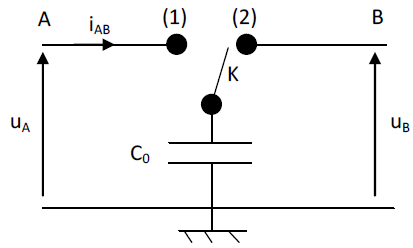
\includegraphics{images/capa_comm.png} 
	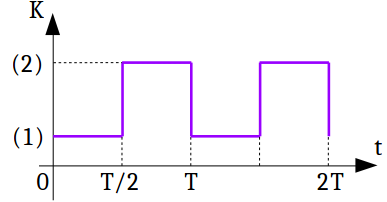
\includegraphics{images/capa_comm_signal.png}
\end{center}

\medskip

\begin{enumerate}
	\item Calculer la charge stockée dans $C_0$ entre les instants 0 et $T/2$, puis entre les instants $T/2$ et $T$.
	\item Quelle quantité de charges passe de A vers B entre les instants 0 et T ?
	\item Calculer alors le courant moyen circulant du point A au point B pendant une période T. 
	\item Donner l'expression de la résistance équivalente $R_{AB}$ vue entre les bornes A et B de cette cellule.
\end{enumerate}

\subsection*{Intégrateur}

On réalise un intégrateur à partir du circuit de la figure 2.

\begin{enumerate}
	\item Donner la fonction de transfert du circuit $T(j\omega) = u_2/u_1$ en fonction de $R_{AB}$ et de $C$.

\begin{center}
	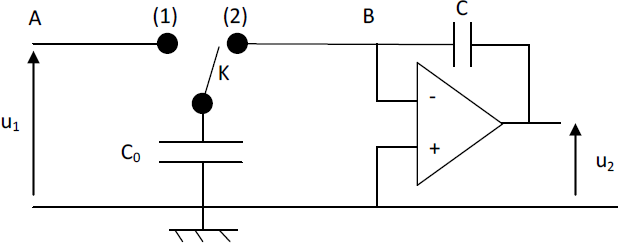
\includegraphics{images/capa_comm_integrateur.png}
\end{center}

	\item Que devient alors la fonction de transfert $T(j\omega{}) = u_2/u_1$ en fonction des éléments du système ($C_0$ et $C$) ?
	\item Quel est l'intérêt d'un tel circuit ?
\end{enumerate}

\subsection*{Etude du MAX296}

On s'intéresse au composant MAX296 dont une partie de la documentation technique est donnée en annexe.

\begin{enumerate}
	\item Quelles sont les fréquences maximales utilisables sur l'entrée \textsc{INPUT} ? Sur l'entrée \textsc{CLOCK} ? Quelles sont les applications visées ?
	\item Quelle fréquence faut-il appliquer sur l'entrée \textsc{CLOCK} pour avoir une fréquence de coupure de 3~kHz ? Que vaut alors l'amplification théorique du signal à : (a) 300~Hz ? (b) 30~kHz ? (c) 5~kHz ?
	\item Avec un filtre du second ordre (type Rauch) avec une pulsation de coupure à la même valeur, quelle aurait été l'amplification : (a) à 30~kHz ? (b) à 5~kHz ?	
	
\end{enumerate}

}

\textbf{Capacité commutée}

\textbf{\textit{1 - Charge stockée dans $C_0$}}

Pour $0 <= t <= T/2$, on a $u_{C0} = u_A$ et $Q_A = C_0 \cdot u_A$.

Pour $T/2 <= t <= T$, on a $u_{C0} = u_B$ et $Q_B = C_0 \cdot u_B$.

\textbf{\textit{2 - Transfert de charges}}

$\Delta{}Q = Q_A - Q_B = C_0 \cdot (u_A - u_B)$

\textbf{\textit{3 - Courant moyen}}

$i_{AB} = \Delta{}Q / T = C_0 \cdot (u_A - u_B) / T = f \cdot C_0 \cdot (u_A - u_B)$

\textbf{\textit{4 - Résistance équivalente}}

$R_{AB} = (u_A - u_B) / i_{AB} = 1 / (f \cdot C_0)$

\medskip

\textbf{Intégrateur}

\textbf{\textit{1 - Fonction de transfert}}

$\frac{u_2}{u_1} = \frac{-Z_C}{R_{AB}}$ avec $Z_C = \frac{1}{j \cdot C \cdot \omega}$

\textbf{\textit{2 - Nouvelle fonction de transfert}}

$$\boxed{T(j\omega) = \frac{C_0 \cdot f}{j \cdot C \cdot \omega}}$$
	
	où $f$ est la fréquence de commutation de l'interrupteur K.

\textbf{\textit{3 - Intérêt}}

On remarque alors que l'on peut piloter la fréquence de transition des intégrateurs par un signal électrique dont on maitrise la fréquence.

\newpage
\textbf{MAX296}

\textbf{\textit{1 - Fréquences et fonctionnement}}

D'après la page 1 de la documentation, sur le MAX296, les signaux d'entrée peuvent aller jusqu'à 50~kHz.

Le signal d'horloge (\textsc{CLOCK}) doit avoir une fréquence 50 fois plus grande que la fréquence de coupure souhaité. On peut donc monter jusqu'à une fréquence de $50 \cdot 50\operatorname{kHz} = 2.5\operatorname{MHz}$.

Ce sont principalement des filtres anti-repliement de spectre prévus pour des applications audio :
\begin{itemize}
	\item spectre : 20~Hz à 20kHz
	\item fréquences d'échantillonnage : 44~kHz
\end{itemize} 

\textbf{\textit{2 - Amplification}}

Il faut appliquer une fréquence de $50 \cdot 3\operatorname{kHz}$, soit 150~kHz.

\medskip

\textbf{A 300~Hz}, le signal est encore dans la bande passante du filtre, il n'est donc pas atténué. Le gain vaut 0~dB, l'amplification vaut donc 1.
	
\medskip

\textbf{A 30~kHz}, le signal a une fréquence ayant une décade d'écart par rapport à la fréquence de coupure du filtre. Le filtre ayant un ordre de 8, le signal perd 160~dB par décade.

	On alors : $G = -160\operatorname{dB}$ ce qui équivaut à $A = 10^{-160/20} = 10^{-8}$.

\medskip
	
\textbf{A 5~kHz}, on est déjà en dehors de la bande passante. La pente est alors de -160dB/décade. On a alors une droite de type : $y = -160 \cdot (log(f) - log(3000))$ (f étant la fréquence recherchée et 3000 étant la fréquence 	de coupure) - on pourra rappeler que $log[K.f] = log[K] + log[f]$.

Ainsi, on a $y = -160 \cdot (log[5000] - log[3000]) = -35\operatorname{dB}$. Et $A = 10^{-35/20} = 0.018$ 


\textbf{\textit{3 - Filtre actif second ordre}}

	Un filtre du second ordre à une décroissance de 40dB/décade en dehors de la bande-passante.

\textbf{A 30~kHz}, le signal a une fréquence ayant une décade d'écart par rapport à la fréquence de coupure du filtre.

	On alors : $G = -40\operatorname{dB}$ ce qui équivaut à $A = 10^{-40/20} = 10^{-2}$.

\medskip
	
\textbf{A 5~kHz}, on est déjà en dehors de la bande passante. La pente est alors de -40dB/décade. On a alors une droite de type : $y = -40 \cdot (log(f) - log(3000))$ (f étant la fréquence recherchée et 3000 étant la fréquence 	de coupure).

Ainsi, on a $y = -40 \cdot (log[5000] - log[3000]) = -8.8\operatorname{dB}$. Et $A = 10^{-8.8/20} = 0.36$.


%%%%%%%%%%%%%%%%%%%

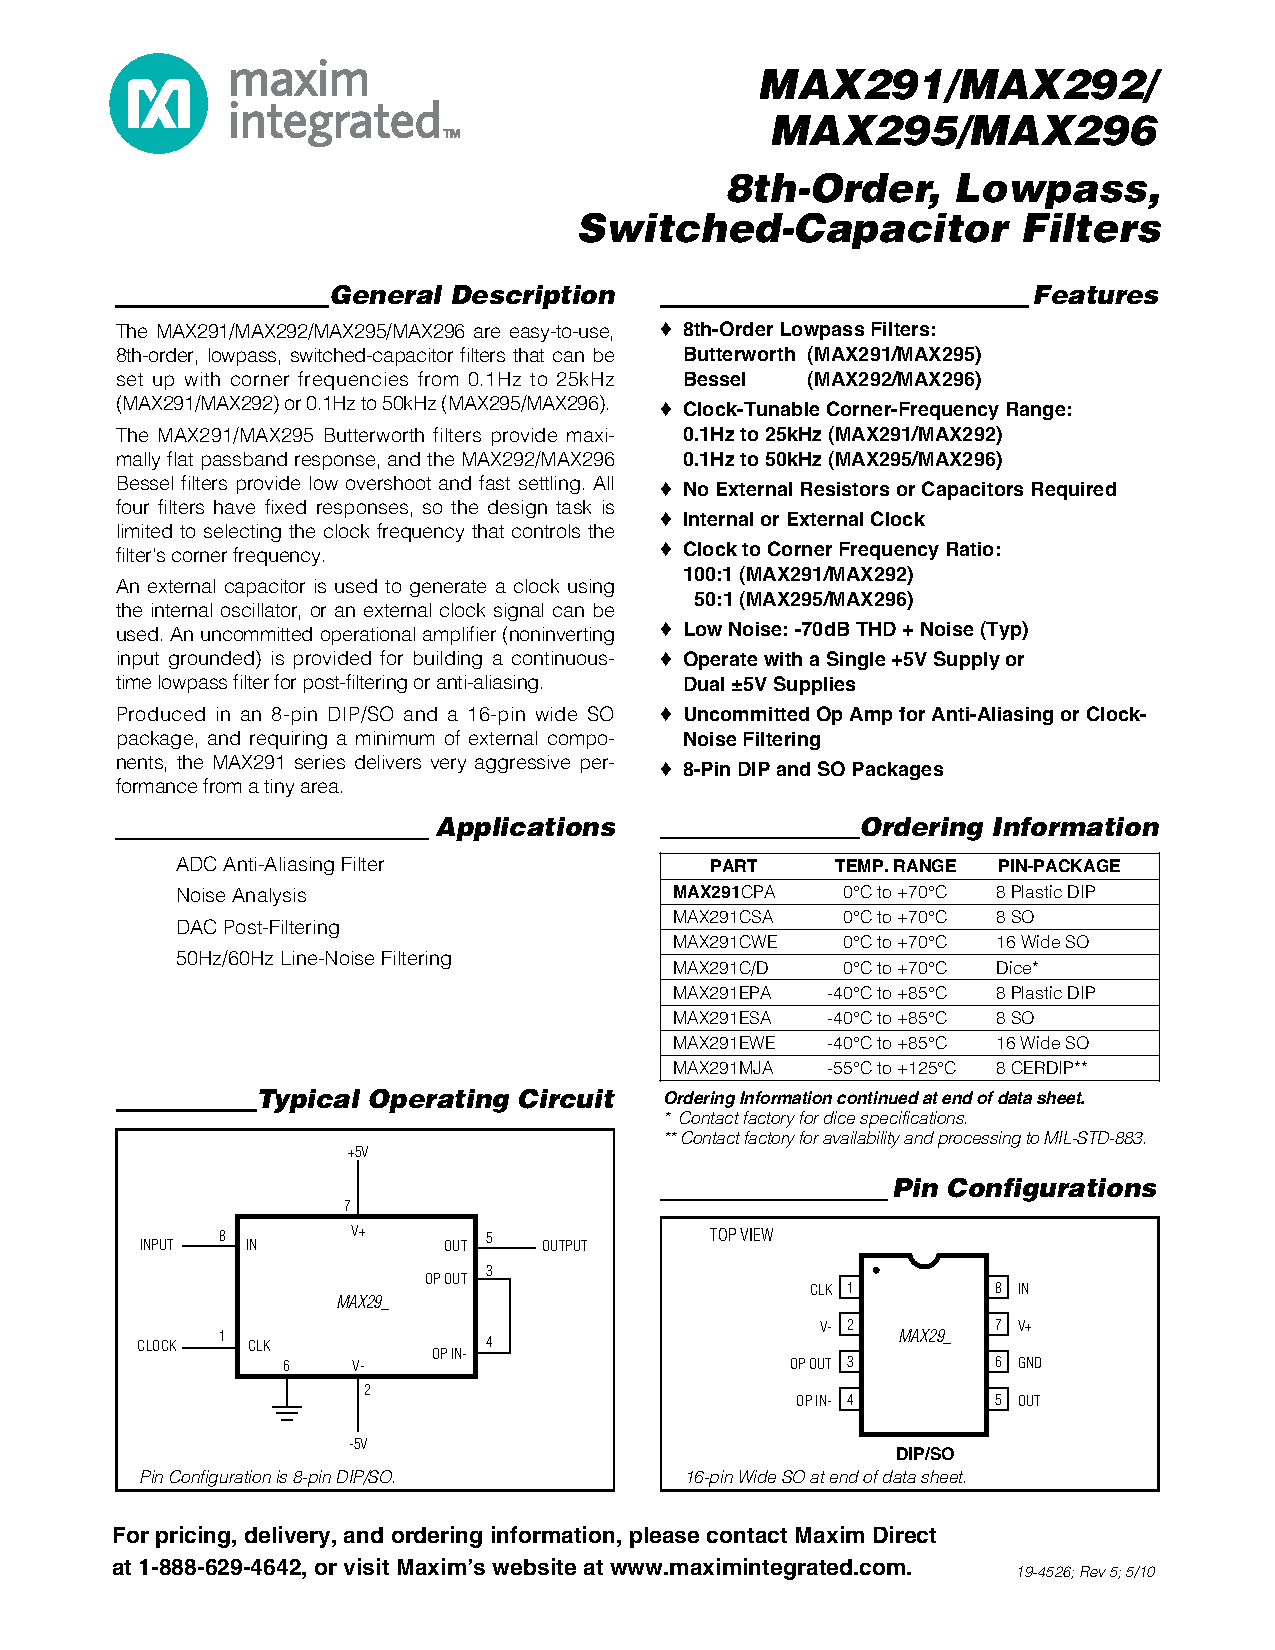
\includepdf[pages=-]{doc/MAX296.pdf}

\newpage
\section*{Annexe : Filtres actif de \textbf{Butterworth} et de \textbf{Chebychev}}

\textit{Document basé sur le cours de Sylvie Lebrun, Filtrage analogique, 2015.}

\subsection*{Gabarit d'un filtre}

Le gabarit d'un filtre correspond aux \textbf{contraintes fréquentielles et en gain} que doit satisfaire le système à développer.

\begin{center}
	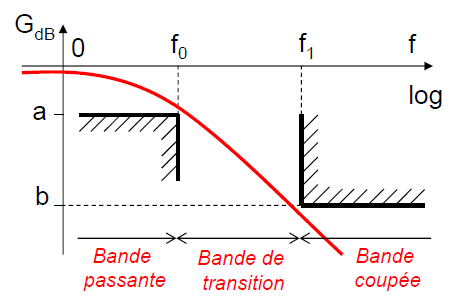
\includegraphics[width=10cm]{images/gabarit_filtre.png}
\end{center}

On souhaite souvent réaliser un système de filtrage qui possède les caractéristiques suivantes :
\begin{itemize}
	\item transmission de fréquence inférieure à $f_0$
	\item valeur minimale $a$ de gain dans la bande de fréquence à transmettre
	\item valeur maximale $b$ de gain dans la bande de fréquence à éliminer (à partir d'une fréquence $f_1$)
\end{itemize}

Le gabarit est caractérisé par 2 points $(f_0, a)$ et $(f_1, b)$.

\medskip

A partir de ce gabarit, plusieurs types de filtres peuvent être utilisés : Butterworth, Chebychev, Bessel, Cauer

\bigskip

Pour la suite, on posera : $X = \frac{\omega}{\omega_c}$ où $\omega_c$ est la fréquence de coupure du système, définie à $-3\operatorname{dB}$ par rapport au gain dans la bande passante.


\begin{center}
	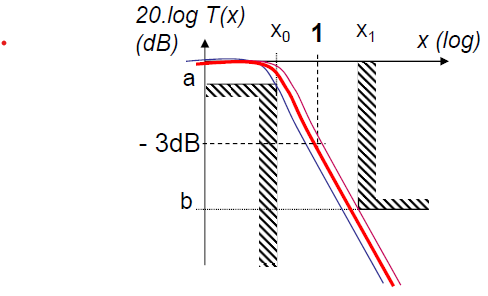
\includegraphics[width=8cm]{images/gabarit_butter.png}
\end{center}

\newpage
\subsection*{Filtre de Butterworth}

Ce type de filtre est utilisé pour sa \textbf{réponse extrêmement plate dans la bande-passante}.


La réponse en fréquence d'un tel filtre est tel que son module vaut :

$$ T(X) = \frac{1}{\sqrt{1 + X^{2\cdot n}}}$$

où $n$ est l'ordre du filtre.

\subsubsection*{Détermination de $n$}
En s'intéressant aux conditions aux limites :


$
\left\{
    \begin{array}{ll}
        20 \cdot \log_{10} T(x_0) > a \\
        20 \cdot \log_{10} T(x_1) < b \\
    \end{array}    
\right. 
$
$\Leftrightarrow$
$
\left\{
    \begin{array}{ll}
        x_0^{2\cdot n} < 10^{-a/10} - 1 & (1)\\
        x_1^{2\cdot n} > 10^{-b/10} - 1 & (2)\\
    \end{array}    
\right. 
$

\medskip

En divisant (2) par (1) on obtient alors la valeur minimale de $n$. On choisira $n$ la plus petite valeur entière qui satisfasse :

$$ n \ge \frac{1}{2} \cdot \frac{\log_{10} \frac{10^{-a/10} - 1}{10^{-b/10} - 1}}{\log_{10} \frac{f_0}{f_1}}$$


\subsubsection*{Détermination de $f_c$}

On calcule alors avec (1) et (2) les fréquences de coupure limites :

$$f_{c,0} = \frac{f_0}{(10^{-a/10} - 1)^{1/(2\cdot n)}} \qquad f_{c,1} = \frac{f_1}{(10^{-b/10} - 1)^{1/(2\cdot n)}}$$

On choisit ensuite la fréquence de coupure comme étant la moyenne géométrique des deux fréquences précédentes :

$$f_c = \sqrt{f_{c,0} \cdot f_{c,1}} $$


\subsubsection*{Fonction de transfert}

Il faut trouver une fraction rationnelle complexe $T(p)$ (avec $p=j\cdot x$) qui admette T(x) comme module. On factorise alors le polynôme : $B_n(x) = 1 + x^{2\cdot n}$. 

On trouve alors que $B_n(p)$ peut s'écrire sous la forme des polynômes obtenus par Butterworth :

\begin{center}
	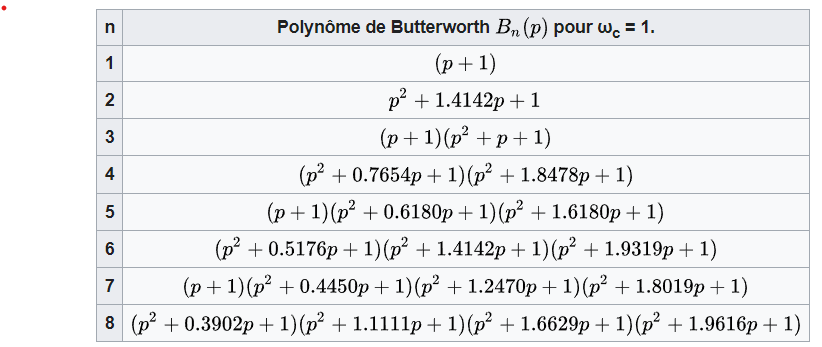
\includegraphics[width=12cm]{images/polynomes_butter.png}
\end{center}


La fonction de transfert normalisée s'écrit alors ($n$ impair et $n$ pair) :

$$ T(p) = \frac{1}{(1 + p) \cdot (a^2 + b^2 + 2\cdot b p + p^2) \cdot (...} \qquad  T(p) = \frac{1}{(a^2 + b^2 + 2\cdot b p + p^2) \cdot (...} $$

\end {document}